\documentclass[11pt,a4paper, 
swedish, english %% Make sure to put the main language last!
]{article}
\pdfoutput=1

%% Andréas's custom package 
%% (Will work for most purposes, but is mainly focused on physics.)
\usepackage{../custom_as}
\usepackage{mathrsfs}
\usepackage{eufrak}
\usepackage{cancel}
%% Figures can now be put in a folder: 
\graphicspath{ {figures/} {script/}%{some_folder_name/}
}
\usepackage{multicol}

%% If you want to change the margins for just the captions
\usepackage[size=small]{caption}

%% To add todo-notes in the pdf
\usepackage[%disable  %%this will hide all notes
]{todonotes} 

%% Change the margin in the documents
\usepackage[
%            top    = 3cm,              %% top margin
%            bottom = 3cm,              %% bottom margin
%            left   = 3cm, right  = 3cm %% left and right margins
]{geometry}

\newcommand{\enull}{\ensuremath{\varepsilon_{0}}}
\newcommand{\lD}{\ensuremath{\lambda_{\text{D}}}}
\newcommand{\wc}{\ensuremath{\omega_{\text{c}}}}
\newcommand{\rhom}{\ensuremath{{\rho_{\text{m}}}}}
\newcommand{\kB}{\ensuremath{k_{\text{B}}}}
\newcommand{\mH}{\ensuremath{m_{\text{H}}}}
\newcommand{\vD}{\ensuremath{v_{\text{D}}}}
\newcommand{\TD}{\ensuremath{T_{\text{D}}}}
\newcommand{\ED}{\ensuremath{E_{\text{D}}}}
\newcommand{\mD}{\ensuremath{m_{\text{D}}}}
\newcommand{\vT}{\ensuremath{v_{\text{T}}}}
\newcommand{\TT}{\ensuremath{T_{\text{T}}}}
\newcommand{\ET}{\ensuremath{E_{\text{T}}}}
\newcommand{\mT}{\ensuremath{m_{\text{T}}}}
\newcommand{\cs}{\ensuremath{c_{\text{s}}}}


%% If you want to chage the formatting of the section headers
\renewcommand{\thesubsection}{\arabic{section}.\Alph{subsection}}



%%%%%%%%%%%%%%%%%%%%%%%%%%%%%%%%%%%%%%%%%%%%%%%%%%%%%%%%%%%%%%%%%%%%%%
\begin{document}%% v v v v v v v v v v v v v v v v v v v v v v v v v v
%%%%%%%%%%%%%%%%%%%%%%%%%%%%%%%%%%%%%%%%%%%%%%%%%%%%%%%%%%%%%%%%%%%%%%


%%%%%%%%%%%%%%%%%%%% vvv Internal title page vvv %%%%%%%%%%%%%%%%%%%%%
\title{Assignment 5 \\
{\Large Plasma Physics -- RRY085}}
\author{Andréas Sundström}
\date\today%{2017-10-15}

\maketitle

%%%%%%%%%%%%%%%%%%%% ^^^ Internal title page ^^^ %%%%%%%%%%%%%%%%%%%%%
%% If you want a list of all todos
%\todolist

\section{Different frames of reference}
In the rest frame of the tritium nucleus the D-T fusion reaction has
its maximum cross section when the incoming deuterium nucleus has an
temperature of around $\TD=\unit[100]{keV}$.
(Note that $\ED\ll\mT c^2\approx\unit[2]{GeV}$ which means that we do
not have to take relativity into account.) That would correspond to an
velocity $\vD$ given by ($\kB=1$)
\begin{equation}
\ED=\frac{1}{2}\mD\vD^2=\alpha^{-1}\TD.
\end{equation}
The constant $\alpha$ is the constant you choose for your
normalization of tempereature, it dosen't matter in the end.

If we instead change to the rest frame of the deuterium nucleus the
tritium nucleus would be rushing in at the same speed $\vT=\vD$, which
would correspond to a temperature of
\begin{equation}
\TD = \alpha \ET = \frac{1}{2}\mT\vT^2
= \frac{1}{2}\qty(\frac{3}{2}\mD)\vD^2 
= \frac{2}{3}\alpha\ED = \frac{2}{3}\TD= \unit[150]{keV}.
\end{equation}
Here we have used the fact that the tritum nucleus basically has
three times the mass of a proton ($\mT=3\mH$) and deuterium is twice
the proton mass ($\mD=2\mH$).

In the lab fram of reference, where the tempereatures are equal
($\TD'=\TT'$), we instead get the equation
\begin{equation}\label{eq1:eqT}
\cancel{\frac{\alpha}{2}}\mD\vD'^2=\cancel{\frac{\alpha}{2}}\mT\vT'^2,
\end{equation}
together with the transformed velocities
\begin{equation}
\vD'=\vD-v_0\qc\quad\vT'=0+v_0.
\end{equation}
With this we can write \eqref{eq1:eqT} as
\begin{equation}
0=\mT v_0^2-\mD(\vD-v_0)^2
=(\mT-\mD)v_0^2 +2\mD\vD v_0 - \mD\vD^2
\end{equation}
which has the solutions
\begin{equation}
v_0=\frac{-\mD\vD\pm
\vD\sqrt{\mD^2+(\mT{-}\mD)\mD}
}{\mT-\mD}
%=\qty(\frac{-2\mH\pm\sqrt{4\mH^2+2\mH^2}}{1\mH})\vD
=\qty(-2\pm\sqrt{6})\vD.
\end{equation}
We are only interested in the plus sign solution, since we want to
transform into a frame of reference where the two nucleons are heading
into each other ``head on''. This means that the tempereature has to
be
\begin{equation}
\TD'=\TT'=\frac{\alpha}{2}\mT v_0^2
=\frac{\alpha}{2}\qty(\frac{3}{2}\mD)\qty(\sqrt6-2)^2\vD^2
=\frac{3}{2}\qty(\sqrt6-2)^2 \TD
\approx\unit[30]{keV}.
\end{equation}






\section{Plasma profiles and ignition}
In this problem, we are concidering volume averages. Assuming that
the only vaiation is along the radius of the toroidal cross section
\begin{equation}\label{eq2:ev}
\ev{x}_V=\frac{2}{a^2}\int_0^a x(r)r\id{r}.
\end{equation}
For the dentity and temperature, we assume that the profile follows
follows this curve
\begin{equation}\label{eq2:xsect}
y(r)=\ev{y}_V\, (1+\nu_y)\qty(1-\frac{r^2}{a^2})^{\nu_y}.
\end{equation}

\subsection*{Check normalisation}
Here we have to check the normalization on \eqref{eq2:xsect}. We are
especially interested in the integral
\begin{equation}\label{eq2:norm}
\int_0^a(1+\nu)\qty(1-\frac{r^2}{a^2})^{\nu}r\id{r}=
\begin{Bmatrix}
  s=1-\frac{r}{a^2}\\
  \rd{s}=-\frac{2r}{a^2}\id{r}
\end{Bmatrix}
=-\frac{a^2}{2} \int_1^0(1+\nu)s^{\nu}\id{s}
=\frac{a^2}{2}.
\end{equation}
This means that indeed \eqref{eq2:xsect} is consitent with \eqref{eq2:ev}.

We can also state another useful result.
\begin{equation}
\begin{aligned}
\ev{n^\xi T^\zeta}_V=&\ev{n}_V^\xi\ev{T}_V^\zeta
\frac{2}{a^2}\int_0^a(1+\nu_n)^\xi(1+\nu_T)^\zeta
\qty(1-\frac{r^2}{a^2})^{\xi\nu_n+\zeta\nu_T}r\id{r}\\
=&\ev{n}_V^\xi\ev{T}_V^\zeta
\frac{(1+\nu_n)^\xi(1+\nu_T)^\zeta}{1+\xi\nu_n+\zeta\nu_T},
\end{aligned}
\end{equation}
which can easily be proven since
\begin{equation}
\frac{2}{a^2}\int_0^a(1+\xi\nu_n+\zeta\nu_T)
\qty(1-\frac{r^2}{a^2})^{\xi\nu_n+\zeta\nu_T}r\id{r}
=1
\end{equation}
by \eqref{eq2:norm}.
This is especially useful for calculating the preasure $P=2nT$,
menaing that we have $\xi=\zeta=1$ giving
\begin{equation}
\ev{P}_V=\ev{n}_V\ev{T}_V
\frac{(1+\nu_n)(1+\nu_T)}{1+\nu_n+\nu_T}.
\end{equation}


\subsection*{Ignition}


\begin{figure}
\centering
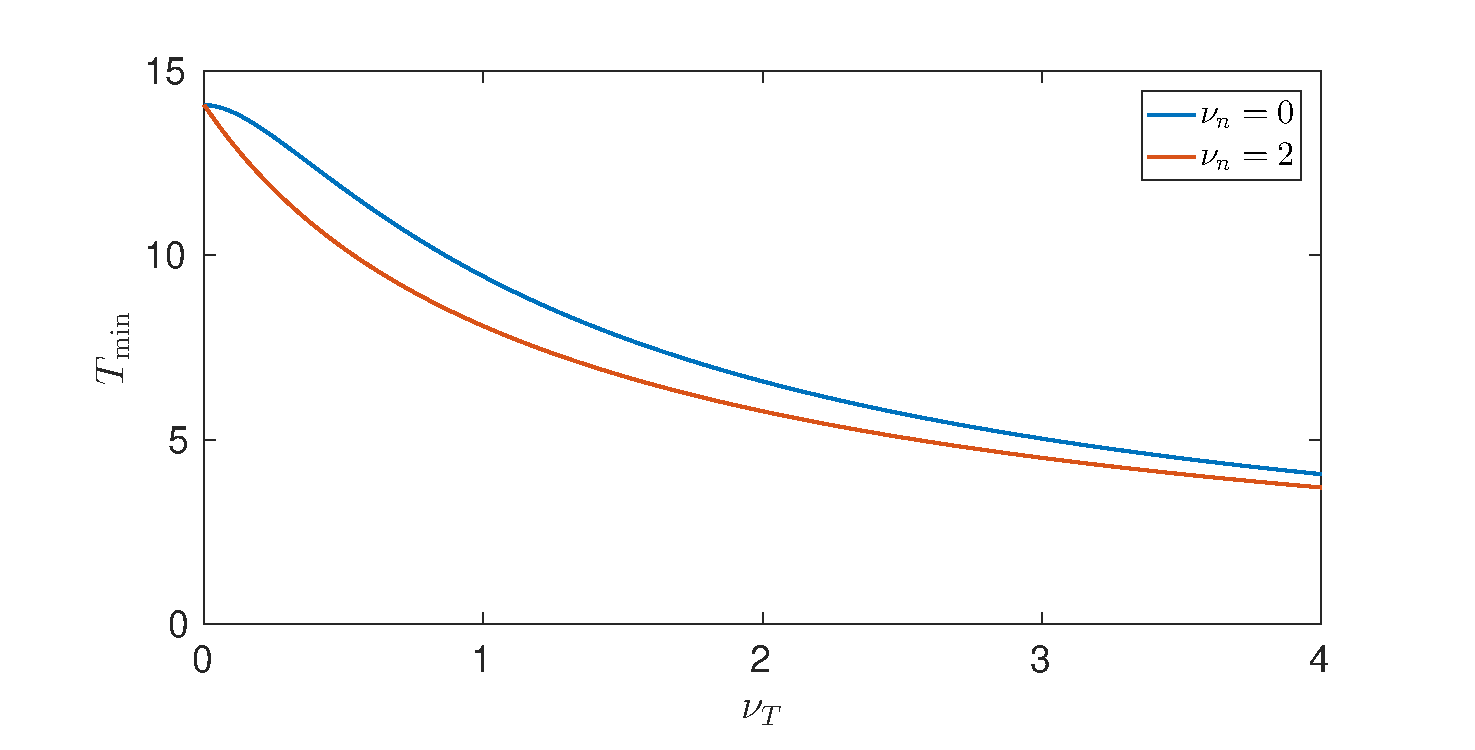
\includegraphics[width=14cm]{T_min.eps}
\caption{}
\label{fig:T_min}
\end{figure}




%%%%%%%%%%%%%%%%%%%%%%%%%%%%%%%%%%%%%%%%%%%%%%%%%%%%%%%%%%%%%%%%%%%%%%
\end{document}%% ^ ^ ^ ^ ^ ^ ^ ^ ^ ^ ^ ^ ^ ^ ^ ^ ^ ^ ^ ^ ^ ^ ^ ^ ^ ^ ^
%%%%%%%%%%%%%%%%%%%%%%%%%%%%%%%%%%%%%%%%%%%%%%%%%%%%%%%%%%%%%%%%%%%%%%
%  LocalWords: Alfvén MHD Bohm quadratically incompressible
%  LocalWords:  logaritmically
